% Options for packages loaded elsewhere
\PassOptionsToPackage{unicode}{hyperref}
\PassOptionsToPackage{hyphens}{url}
%
\documentclass[
]{article}
\usepackage{amsmath,amssymb}
\usepackage{lmodern}
\usepackage{iftex}
\ifPDFTeX
  \usepackage[T1]{fontenc}
  \usepackage[utf8]{inputenc}
  \usepackage{textcomp} % provide euro and other symbols
\else % if luatex or xetex
  \usepackage{unicode-math}
  \defaultfontfeatures{Scale=MatchLowercase}
  \defaultfontfeatures[\rmfamily]{Ligatures=TeX,Scale=1}
\fi
% Use upquote if available, for straight quotes in verbatim environments
\IfFileExists{upquote.sty}{\usepackage{upquote}}{}
\IfFileExists{microtype.sty}{% use microtype if available
  \usepackage[]{microtype}
  \UseMicrotypeSet[protrusion]{basicmath} % disable protrusion for tt fonts
}{}
\makeatletter
\@ifundefined{KOMAClassName}{% if non-KOMA class
  \IfFileExists{parskip.sty}{%
    \usepackage{parskip}
  }{% else
    \setlength{\parindent}{0pt}
    \setlength{\parskip}{6pt plus 2pt minus 1pt}}
}{% if KOMA class
  \KOMAoptions{parskip=half}}
\makeatother
\usepackage{xcolor}
\usepackage[margin=1in]{geometry}
\usepackage{graphicx}
\makeatletter
\def\maxwidth{\ifdim\Gin@nat@width>\linewidth\linewidth\else\Gin@nat@width\fi}
\def\maxheight{\ifdim\Gin@nat@height>\textheight\textheight\else\Gin@nat@height\fi}
\makeatother
% Scale images if necessary, so that they will not overflow the page
% margins by default, and it is still possible to overwrite the defaults
% using explicit options in \includegraphics[width, height, ...]{}
\setkeys{Gin}{width=\maxwidth,height=\maxheight,keepaspectratio}
% Set default figure placement to htbp
\makeatletter
\def\fps@figure{htbp}
\makeatother
\setlength{\emergencystretch}{3em} % prevent overfull lines
\providecommand{\tightlist}{%
  \setlength{\itemsep}{0pt}\setlength{\parskip}{0pt}}
\setcounter{secnumdepth}{-\maxdimen} % remove section numbering
\usepackage{helvet} \renewcommand\familydefault{\sfdefault}
\usepackage{booktabs}
\usepackage{longtable}
\usepackage{array}
\usepackage{multirow}
\usepackage{wrapfig}
\usepackage{float}
\usepackage{colortbl}
\usepackage{pdflscape}
\usepackage{tabu}
\usepackage{threeparttable}
\usepackage{threeparttablex}
\usepackage[normalem]{ulem}
\usepackage{makecell}
\usepackage{xcolor}
\ifLuaTeX
  \usepackage{selnolig}  % disable illegal ligatures
\fi
\IfFileExists{bookmark.sty}{\usepackage{bookmark}}{\usepackage{hyperref}}
\IfFileExists{xurl.sty}{\usepackage{xurl}}{} % add URL line breaks if available
\urlstyle{same} % disable monospaced font for URLs
\hypersetup{
  pdftitle={Lista 1 modulo 3},
  pdfauthor={César A. Galvão - 19/0011572},
  hidelinks,
  pdfcreator={LaTeX via pandoc}}

\title{Lista 1 modulo 3}
\author{César A. Galvão - 19/0011572}
\date{2022-09-20}

\begin{document}
\maketitle

\newpage{}

{
\setcounter{tocdepth}{3}
\tableofcontents
}
\let\oldsection\section
\renewcommand\section{\clearpage\oldsection}

\hypertarget{section}{%
\section{}\label{section}}

\hypertarget{modelo-e-anova}{%
\subsection{Modelo e ANOVA}\label{modelo-e-anova}}

É utilizado o modelo de experimentos fatoriais, representado por:

\begin{align*}
  y_{ijk} = \mu + \tau_i + \beta_j + \left( \tau\beta \right)_{ij} + e_{ijk}, \quad i = 1, 2,..., a; \quad j = 1, 2,..., b \quad k = 1, 2,..., n
\end{align*}

em que \(\mu\) é a média geral, \(\tau_i\) é o efeito do fator
\textbf{vidro}, \(\beta_j\) é o efeito do fator \textbf{fósforo},
\((\tau\beta)_{ij}\) é o efeito de interação entre os dois fatores e
\(e_{ijk}\) é o desvio do elemento. Portanto, existem
\(a \cdot b = 3 \cdot 2 = 6\) tratamentos possíveis para este
experimento.

\begin{longtable}{cccccc}
\toprule
term & df & sumsq & meansq & statistic & p.value\\
\midrule
\endfirsthead
\multicolumn{6}{@{}l}{\textit{(continued)}}\\
\toprule
term & df & sumsq & meansq & statistic & p.value\\
\midrule
\endhead

\endfoot
\bottomrule
\endlastfoot
\cellcolor{gray!15}{phosphor} & \cellcolor{gray!15}{2} & \cellcolor{gray!15}{933.3333} & \cellcolor{gray!15}{466.6667} & \cellcolor{gray!15}{8.8421} & \cellcolor{gray!15}{0.0044}\\
glass & 1 & 14450.0000 & 14450.0000 & 273.7895 & 0.0000\\
\cellcolor{gray!15}{phosphor:glass} & \cellcolor{gray!15}{2} & \cellcolor{gray!15}{133.3333} & \cellcolor{gray!15}{66.6667} & \cellcolor{gray!15}{1.2632} & \cellcolor{gray!15}{0.3178}\\
Residuals & 12 & 633.3333 & 52.7778 & NA & NA\\*
\end{longtable}

Pela tabela de ANOVA, os efeitos de ambos os fatores do experimento são
significativos considerando mesmo \(\alpha = 0,01\). No entanto
rejeita-se a hipótese de existência de interação entre os fatores. Ou
seja, pode-se considerar os efeitos do tipo de vidro e do tipo de
fósforo independentes.

\hypertarget{estimadores}{%
\subsection{Estimadores}\label{estimadores}}

\begin{longtable}{cc}
\toprule
$\mu$ & $\sigma^2$\\
\midrule
\endfirsthead
\multicolumn{2}{@{}l}{\textit{(continued)}}\\
\toprule
$\mu$ & $\sigma^2$\\
\midrule
\endhead

\endfoot
\bottomrule
\endlastfoot
\cellcolor{gray!15}{263.333} & \cellcolor{gray!15}{52.778}\\*
\end{longtable}

\begin{longtable}{cc}
\toprule
$\tau_1$ & $\tau_2$\\
\midrule
\endfirsthead
\multicolumn{2}{@{}l}{\textit{(continued)}}\\
\toprule
$\tau_1$ & $\tau_2$\\
\midrule
\endhead

\endfoot
\bottomrule
\endlastfoot
\cellcolor{gray!15}{28.333} & \cellcolor{gray!15}{-28.333}\\*
\end{longtable}

\begin{longtable}{ccc}
\toprule
$\beta_1$ & $\beta_2$ & $\beta_3$\\
\midrule
\endfirsthead
\multicolumn{3}{@{}l}{\textit{(continued)}}\\
\toprule
$\beta_1$ & $\beta_2$ & $\beta_3$\\
\midrule
\endhead

\endfoot
\bottomrule
\endlastfoot
\cellcolor{gray!15}{-3.333} & \cellcolor{gray!15}{10} & \cellcolor{gray!15}{-6.667}\\*
\end{longtable}

\begin{longtable}{cccccc}
\toprule
$\tau_1\beta_1$ & $\tau_1\beta_2$ & $\tau_1\beta_3$ & $\tau_2\beta_1$ & $\tau_2\beta_2$ & $\tau_2\beta_3$\\
\midrule
\endfirsthead
\multicolumn{6}{@{}l}{\textit{(continued)}}\\
\toprule
$\tau_1\beta_1$ & $\tau_1\beta_2$ & $\tau_1\beta_3$ & $\tau_2\beta_1$ & $\tau_2\beta_2$ & $\tau_2\beta_3$\\
\midrule
\endhead

\endfoot
\bottomrule
\endlastfoot
\cellcolor{gray!15}{21.667} & \cellcolor{gray!15}{38.333} & \cellcolor{gray!15}{25} & \cellcolor{gray!15}{-28.333} & \cellcolor{gray!15}{-18.333} & \cellcolor{gray!15}{-38.333}\\*
\end{longtable}

\hypertarget{gruxe1ficos-de-interauxe7uxe3o}{%
\subsection{Gráficos de
interação}\label{gruxe1ficos-de-interauxe7uxe3o}}

As linhas paralelas do gráfico a seguir sugerem não haver interação
entre os fatores, além de indicar possível diferença entre o fósfóro
tipo 2 e os demais para vidro tipo 1.

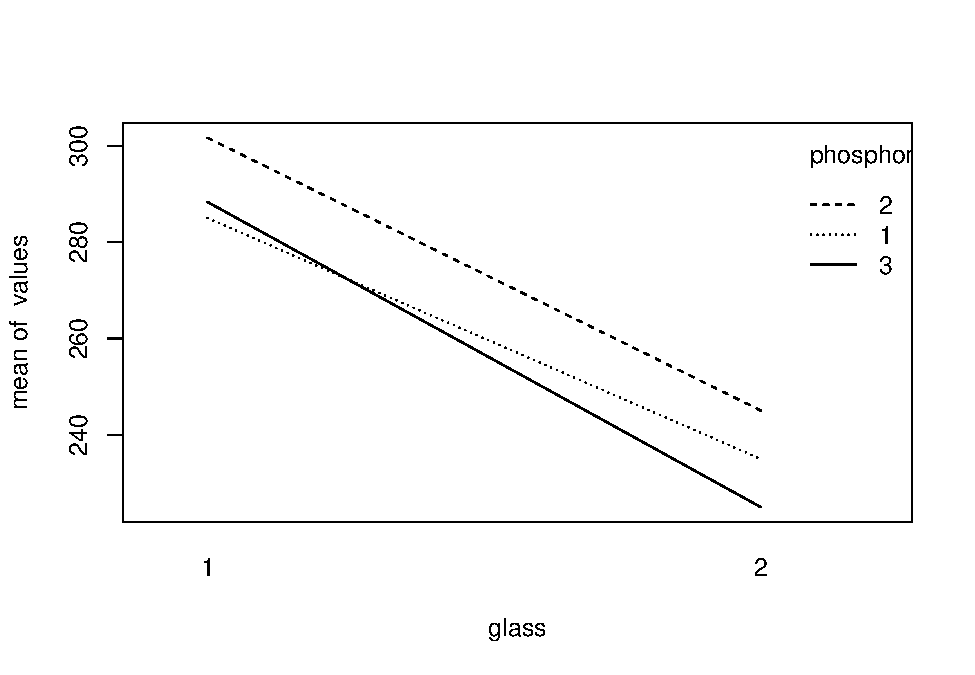
\includegraphics{lista8_files/figure-latex/grafico1-1.pdf}

O gráfico seguinte também sugere não haver interação entre fatores, mas
aparentemente deve haver uma diferença de desempenho quanto ao tipo de
vidro, independentemente do tipo de fósforo.

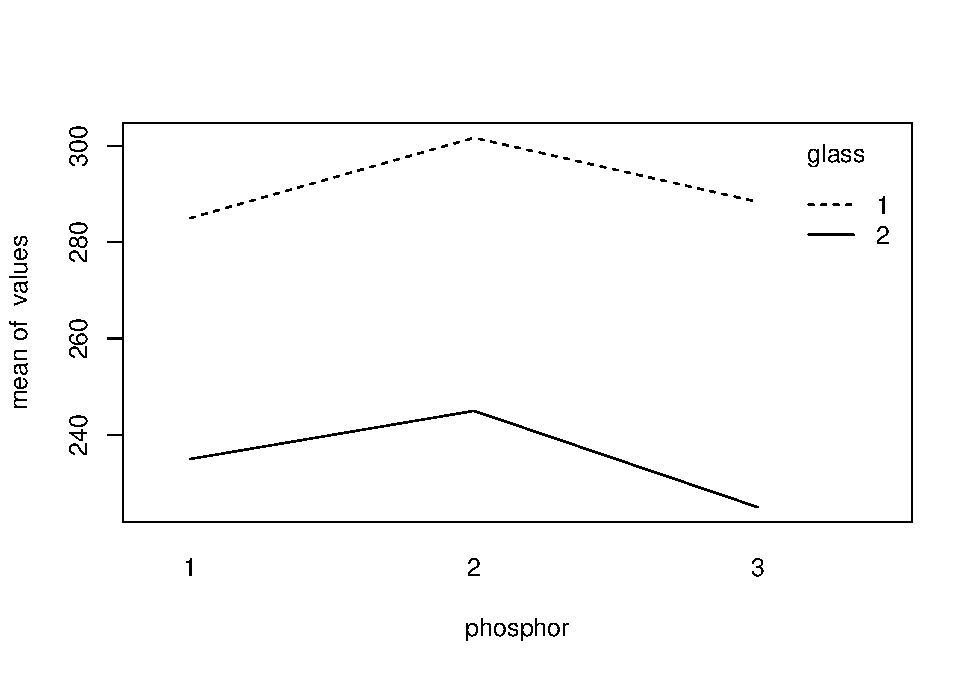
\includegraphics{lista8_files/figure-latex/grafico2-1.pdf}

\hypertarget{decomposiuxe7uxe3o-de-graus-de-liberdade}{%
\subsection{Decomposição de graus de
liberdade}\label{decomposiuxe7uxe3o-de-graus-de-liberdade}}

A seguir são decompostos os graus de liberdade para o tipo de fósforo,
quando o tipo de vidro é 1.

\hypertarget{teste-f}{%
\subsubsection{Teste F}\label{teste-f}}

A seguir, o teste F é realizado para os tipos de fósforo quando o tipo
do vidro é 1. Considera-se \(H_0\) como a igualdade entre efeitos de
fósforo e \(H_1\) a diferença de pelo menos um nível em relação aos
demais. O p-valor do teste é calculado da seguinte forma:

\begin{align*}
  \text{p-valor} = 1-F\left( \frac{QM_{\text{fosf-1}}}{QM_{\text{res}}}, gl1 = 2, gl2 = 12 \right)
\end{align*}

\begin{verbatim}
##                       Df Sum Sq Mean Sq F value Pr(>F)  
## dados_vidro1$phosphor  2  466.7  233.33   7.636 0.0224 *
## Residuals              6  183.3   30.56                 
## ---
## Signif. codes:  0 '***' 0.001 '**' 0.01 '*' 0.05 '.' 0.1 ' ' 1
\end{verbatim}

Obtém-se p-valor igual a 0.0364, o que sugere que há de fato diferença
entre os níveis de resposta quando se considera apenas o vidro tipo 1.

\hypertarget{tukey}{%
\subsubsection{Tukey}\label{tukey}}

O teste de Tukey é realizado utilizando a função \texttt{TukeyHDS()} e
os resultados são expostos abaixo. Da mesma forma, a hipótese nula é
rejeitada e diz-se que não há diferença entre os trsão superiores
àqueles do teste F.

\begin{longtable}{cccccc}
\toprule
term & contrast & estimate & conf.low & conf.high & adj.p.value\\
\midrule
\endfirsthead
\multicolumn{6}{@{}l}{\textit{(continued)}}\\
\toprule
term & contrast & estimate & conf.low & conf.high & adj.p.value\\
\midrule
\endhead

\endfoot
\bottomrule
\endlastfoot
\cellcolor{gray!15}{phosphor:glass} & \cellcolor{gray!15}{2:1-1:1} & \cellcolor{gray!15}{16.6667} & \cellcolor{gray!15}{-3.2575} & \cellcolor{gray!15}{36.5908} & \cellcolor{gray!15}{0.1230}\\
phosphor:glass & 3:1-1:1 & 3.3333 & -16.5908 & 23.2575 & 0.9918\\
\cellcolor{gray!15}{phosphor:glass} & \cellcolor{gray!15}{3:1-2:1} & \cellcolor{gray!15}{-13.3333} & \cellcolor{gray!15}{-33.2575} & \cellcolor{gray!15}{6.5908} & \cellcolor{gray!15}{0.2855}\\*
\end{longtable}

\hypertarget{probabilidade-de-erro-tipo-ii-para-vidros}{%
\subsection{Probabilidade de erro tipo II para
vidros}\label{probabilidade-de-erro-tipo-ii-para-vidros}}

Calcula-se a probabilidade de erro tipo 2 considerando:

\begin{itemize}
\tightlist
\item
  \(\tau = \{20, -20\}\);
\item
  \(n = 3, a = 2, b = 3\);
\item
  \(\phi^2 = nb \frac{\sum \tau^2}{QM_\text{res}}\);
\item
  \(F_{crit} = \frac{QM_{\text{vidro}}}{QM_{\text{Res}}}\) =
  14450/52.778 = 273.7895;
\end{itemize}

Obtém-se erro tipo II igual a 0.907.

\end{document}
